\section{Memory Efficient Convolutions}
\begin{figure}
	\centering
	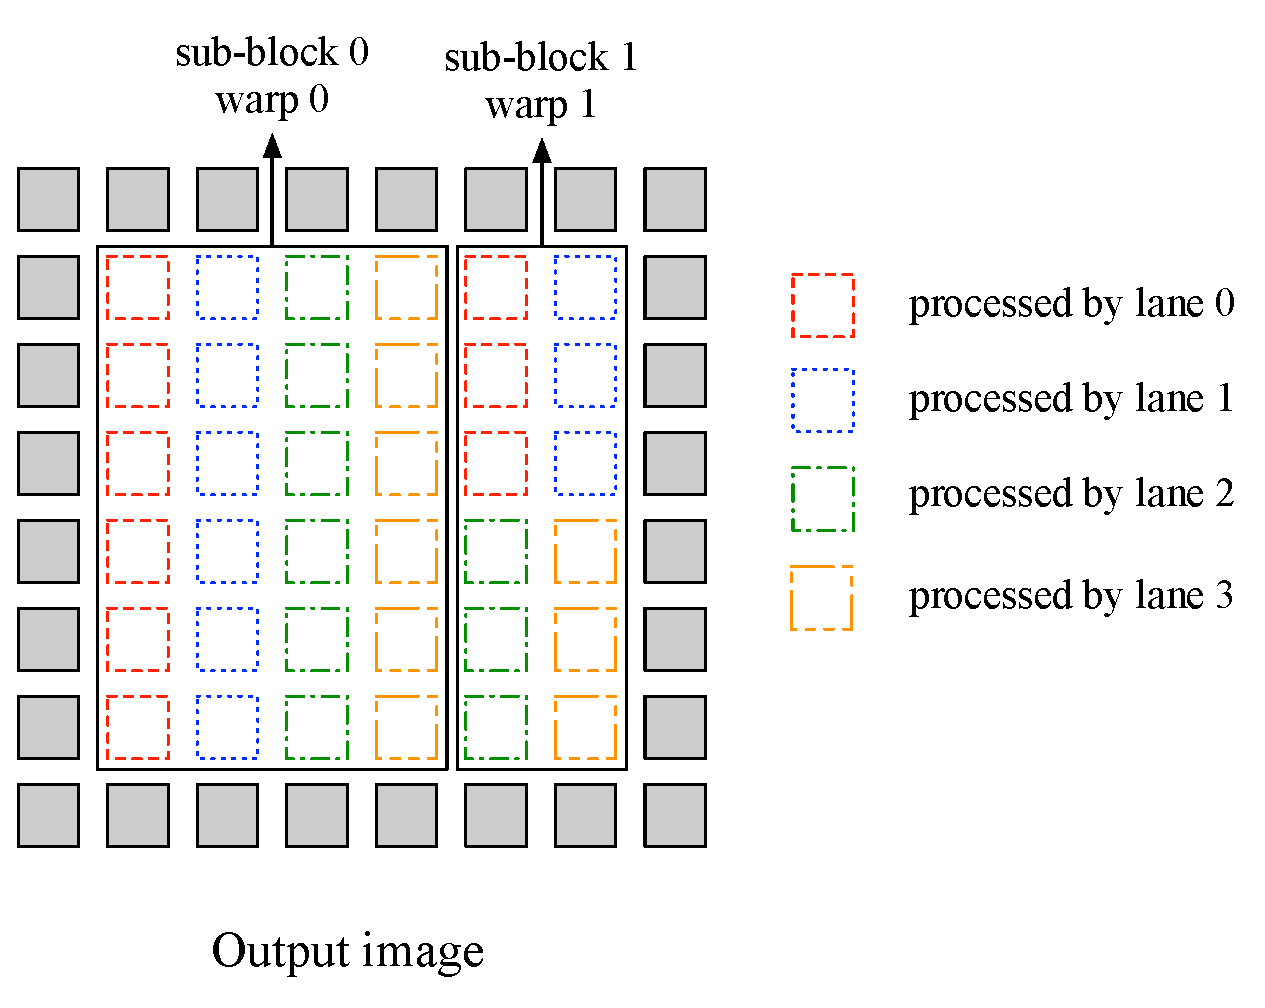
\includegraphics[width=0.9\columnwidth,height=5.5cm]{./figure/overalldesign.eps}
\caption{The output is produced by sliding a $3 \times 3$ filter over an $8 \times 8$ input with one pad. Edge elements and inner elements are processed by different {\color{red}thread blocks}. We assume that {\color{red}warp size} is 4 and thus $laneid=threadid\%4$.}
\label{fig:overalldesign}
\end{figure}


In this section, we demonstrate how to employ our two reuse algorithms on 2D and 3D convolutions. The main difference between
implementations of 2D and 3D convolutions is how to load filters. For 2D convolution, we focus on the scenario where a filter is used to
slide over a large image. Therefore, we can load the entire filter into shared memory and one thread block only needs to load the
filter once. For 3D convolution, we focus on the scenario where many filters are used to slide over a batch of images. This is often the
first layer of CNNs. The entire filters normally can not fit into the shared memory, thus we need to load filters multiple times.

To make this easily understood, we use 2D convolution {\color{red}running at NVIDIA GPU} as an example for illustration. In our implementation, we first divide the output
into sub-blocks and each sub-block contains exactly 32 ({\color{red}warp size}) columns except for the last sub-block which may contain less columns.
Each {\color{red}thread block} processes one or more sub-blocks and each warp process one sub-block. Threads within the same warp process adjacent
columns of one sub-block.
\begin{algorithm}
	\KwIn{$I$, $F$, $O$, $subBlockHeight$}
	\KwOut{$O$}
	load filter into shared memory\;
	$\_\_syncthreads()$\;
	\If{$blockIdx.x \textless gridDim.x-1$}{
		Calculate the index of the first input element this thread needs, denoted as $baseIndex$\;
		\For{$i \gets 0$ \KwTo $I_C$}{
			$inputIndex \gets baseIndex+i*I_H*I_W$\;
			\For{$j \gets 0$ \KwTo $subBlockHeight$}{
				Use Algorithm \ref{algo:basic} and Algorithm \ref{algo:basic2} to load input elements the thread needs, the loaded elements are denoted as $row$\;
				
				Use Algorithm \ref{algo:rowreuse} to calculate output elements and store results into thread local register array $sum$\;
			}
		}
		Write array $sum$ into global memory\;
	}
	\Else{
		Process the remaining inner elements of $O$\;
		Process the edge elements of $O$\;
	}
	\caption{Overall design}
	\label{algo:overalldesign}
\end{algorithm}

Figure \ref{fig:overalldesign} is an illustration of how to map threads onto output elements. Since 2D convolution normally produces
an output image of the same size as the input image, therefore we need to pad the input image. But we do not actually allocate memory on
GPU, instead we use different methods to calculate edge and inner elements of the output image. In Figure \ref{fig:overalldesign}, edge
elements and inner elements are denoted as shaded squares and dashed squares respectively.

We demonstrate how to deal with inner elements in this paper and we calculate edge elements with a similar method as inner elements. In
Figure \ref{fig:overalldesign}, we assume that each {\color{red}warp} contains 4 threads. We can see that the inner elements are divided into two
sub-blocks. Sub-block 0 contains 4 columns which is exactly the {\color{red}warp size}. Sub-block 1 contains only 2 columns, to make full use of threads
within a {\color{red}warp}, we divide the last two columns evenly among 4 threads. A generalized overall design is shown in Algorithm
\ref{algo:overalldesign}.

In Algorithm \ref{algo:overalldesign}, we first load the filter into shared memory (Line 1-2). Then we process sub-blocks with exact 32
columns in Line 3-13 and the last sub-block in Line 14-17. Each thread calculates one column of output elements as follows: First, each
thread calculates the address of the first input element it needs (Line 4-6); Second, each thread uses Algorithm \ref{algo:basic} and
Algorithm \ref{algo:basic2} to fulfill the vector $row$ which contains a row of the sub-block (Line 8); Third, each thread passes the
vector $row$ to Algorithm \ref{algo:rowreuse} to calculate multiple output elements and store results in register array $sum$ (Line 9);
Last, each thread writes the result array $sum$ into global memory (Line 12).
